
Google Docs made real-time editing in browsers easy for millions of
users. However, Google mediates real-time editing sessions with
central servers raising issues on privacy, censorship, economic
intelligence. It also raises scalability issues in term of number of
participants.  Despite that small groups currently constitute the main
range of users, events such as massive online lectures, TV shows,
conferences gather larger groups.  Google Docs supports large groups
but only the first fifty users can edit, next users have their rights
limited to document reading. We think that real-time editors should allow
editing at anytime and anywhere, whatever the number of
participants.

%% In this paper we focus on building a real-time editor that supports privacy
%% and that adapts \TODO{gently} from small groups to large groups

Decentralized real-time editors~\cite{oster2006data, sun1998operational,
  sun2009contextbased} do not require intermediate servers and by the same
settle privacy issues. However, scalability issues remain.  Addressing
scalability requires finding a good trade-off between communication, space and
time complexities. Achieving a sublinear communication complexity compared to
the number of participants is crucial for supporting large groups.

%% But consistency maintenance of documents requires each message to piggyback
%% additional information which greatly impacts the communication complexity.

To provide availability and responsiveness of documents, real-time editors use
the optimistic replication. As such, each user creates a local copy of the
document and directly performs her modification on it. Changes are broadcast to
all replica owners where they are integrated. Strong eventual consistency states
that replicas integrating an identical set of operations converge to an
equivalent state, i.e., users read a same document.

Decentralized algorithms of Operational
Transformation~\cite{sun2009contextbased} (OT) require piggybacking a
state or a context vector in order to detect concurrent
operations. Unfortunately, state vectors grow linearly compared to the
number of members that ever participated in the authoring. Hence,
these approaches behave great with stable small groups of users, but
poorly scale to highly dynamic large group of users and high latency.

Conflict-Free Replicated Data Types~\cite{shapiro2011comprehensive}
(CRDTs) avoid paying the price of concurrency detection by providing
commutative operations. However, they require to piggyback unique and
immutable identifiers to every operation broadcast on the network. The
size of this identifier is the key for the communication complexity
and consequently the scalability of the approach. Two classes of CRDTs
designed for sequences exist:
\begin{itemize}
\item CRDTs such as WOOT~\cite{oster2006data} piggyback a
  constant-size identifer which is optimal. However, it requires to
  keep tombstones ie. mark removed elements from the structure and
  hide them from the users. A document may appear empty while storing
  thousands of unnecessary elements. Tombstones degrades time
  complexity for integrating operations and can make the real-time editor
  unusable. Removing tombstones require a costly garbage collecting
  algorithms that can hardly be deployed in such context.
\item CRDTs such as Logoot~\cite{weiss2010logootundo} do not require tombtones but
  piggyback variable size identifiers. Depending on the identifier
  allocation strategy, they may grow linearly with the document
  size and degrades quickly the communication complexity. The
  replicated structure eventually need an unaffordable balancing
  mechanism.

  The allocation strategy \LSEQ~\cite{nedelec2013concurrency} aims to
  avoid such balancing mechanism by sublinearly upper-bounding the
  space complexity of its identifiers. It conjectured a
  polylogarithmic growth of the identifiers size
  $\mathcal{O}((\log d)^2)$ where $d$ is the document
  size. %Experiments empirically confirmed the conjecture.
\end{itemize}

The contributions of  this paper are threefold:
\begin{itemize}
\item Compared to previous work~\cite{nedelec2013concurrency} , we
  demonstrate the upper bounds on space and time complexities of
  LSeq. This result opens the way for building decentralized and
  scalable real-time editors. % we thoroughly analyze the \LSEQ's
  % complexity in time, space and communication. In particular, we
  % isolate three editing behaviors: left-to-right, right-to-left, and
  % random -- real-life editing being a composition of these
  % three. \LSEQ sacrifices on its worst-case complexity which
  % \TODO{rarely} happens to improve the identifiers size of common
  % editing behaviors. They become polylogarithmically upper-bounded
  % compared to the document size.
\item We describe all the outlines to develop a distributed
  collaborative editor for massive editing of large documents.
\item We built a real-time decentralized editor running in web
  browser\footnote{\url{https://github.com/Chat-Wane/CRATE}}. In the Grid'5000
  testbed, we launched an editing session involving up till 600 connected
  browsers. The resulting documents reach millions of
  characters. Figure~\ref{fig:traffic} shows the result of the experiment. We
  observe that the traffic generated grows following $\ln N (\log d)^2$ where
  $N$ is the network size, $\ln N$ is a multiplicative factor brought by
  scalable broadcast~\cite{nedelec2015spray}, $d$ is the document size, and $(\log d)^2$ is
  brought by the messages piggybacking \LSEQ's identifiers.
\end{itemize}

\begin{figure}
  \centering
  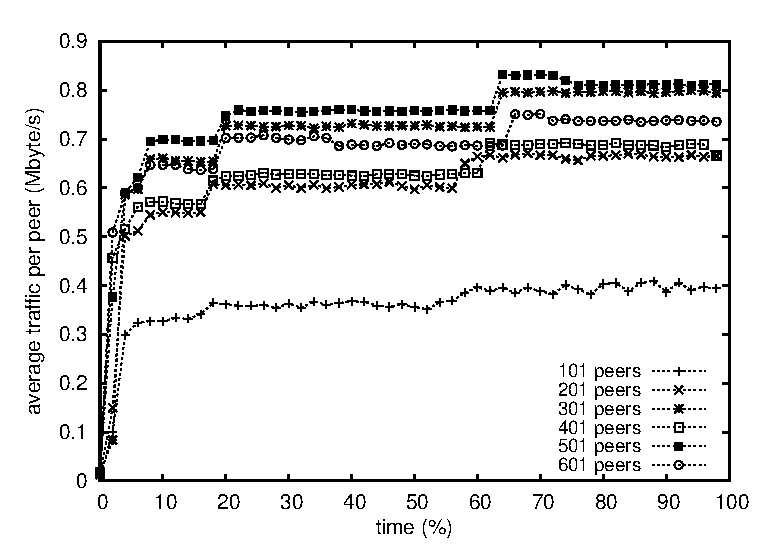
\includegraphics[width=0.8\textwidth]{img/traffic.eps}
  \caption{\label{fig:traffic} Traffic generated by editing sessions of
    various size.}
\end{figure}

%%% Local Variables: 
%%% mode: latex
%%% TeX-master: "../paper"
%%% End: 
